\documentclass{standalone}
\usepackage{pgf}
\usepackage{amsmath}
\usepackage{tikz}
\usetikzlibrary{shapes,arrows}
\usetikzlibrary{positioning}
\usepackage{tikz}
\usetikzlibrary{positioning}
\usetikzlibrary{shapes.geometric}
\usetikzlibrary{shapes.misc}
\usepackage{amsmath}
\usepackage{amssymb}
\usepackage{xstring}


\begin{document}
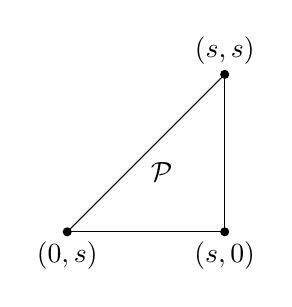
\begin{tikzpicture}
 \draw (0,0) -- (2,0);
 \draw (0,0) -- (2,2);
 \draw (2,0) -- (2,2); 

 \draw [fill=black] (0,-0.) circle (0.05) node[below, black]{$(0,s)$};
  \draw [fill=black] (2,-0.) circle (0.05) node[below, black]{$(s,0)$};
 \draw [fill=black] (2,2.) circle (0.05) node[above, black]{$(s,s)$};

  \draw (1.2,1.0) node[anchor=north] {$\mathcal{P}$};    

 \end{tikzpicture}
\end{document}
